\documentclass{standalone}
\usepackage{tikz}
\usetikzlibrary{patterns}
\usetikzlibrary{positioning}
\usetikzlibrary{patterns, positioning}
\usetikzlibrary{shapes.misc}
\usepackage[outline]{contour}
\contourlength{1.5pt} 
\usetikzlibrary{calc}
        \usepackage{relsize}
        \tikzset{fontscale/.style = {font=\relsize{#1}}}

\begin{document}
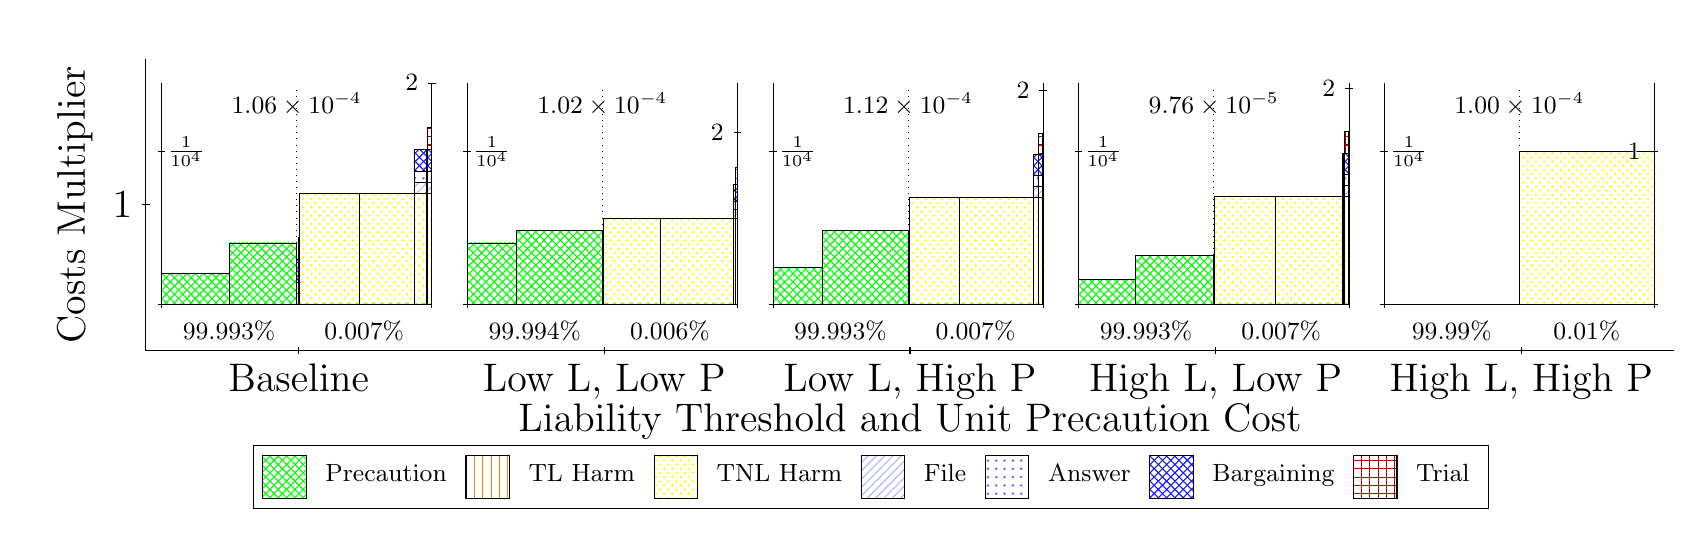
\begin{tikzpicture}
\clip(-0.5,-1.1) rectangle +(20.91,6.2);
\draw[black] (1,1) -- (1,4.7);
\node[rotate=90, fontscale=2, anchor=center] at (0.1, 2.85) {Costs Multiplier};
\draw[black] (0.95,2.85) -- (1.05,2.85);
\node[fontscale=2, anchor=east] at (0.95, 2.85) {1};

\draw[black] (1,1) -- (20.41,1);
\node[fontscale=2, anchor=center] at (10.705, 0.1) {Liability Threshold and Unit Precaution Cost};
\draw[black] (2.941,0.95) -- (2.941,1.05);
\node[fontscale=2, anchor=north] at (2.941, 0.95) {Baseline};
\draw[black] (6.823,0.95) -- (6.823,1.05);
\node[fontscale=2, anchor=north] at (6.823, 0.95) {Low L, Low P};
\draw[black] (10.705,0.95) -- (10.705,1.05);
\node[fontscale=2, anchor=north] at (10.705, 0.95) {Low L, High P};
\draw[black] (14.587,0.95) -- (14.587,1.05);
\node[fontscale=2, anchor=north] at (14.587, 0.95) {High L, Low P};
\draw[black] (18.469,0.95) -- (18.469,1.05);
\node[fontscale=2, anchor=north] at (18.469, 0.95) {High L, High P};


\draw[pattern=crosshatch, pattern color=green,draw=black,very thin] (1.2,1.592) rectangle (2.058,1.9791);
\draw[pattern=crosshatch, pattern color=green,draw=black,very thin] (2.058,1.592) rectangle (2.916,2.3662);
\draw[pattern=crosshatch, pattern color=green,draw=black,very thin] (2.916,1.592) rectangle (2.9373,1.592);
\draw[pattern=north east lines, pattern color=blue!30,draw=black,very thin] (2.916,1.592) rectangle (2.9373,1.7324);
\draw[pattern=dots,  pattern color=blue!60,draw=black,very thin] (2.916,1.7324) rectangle (2.9373,1.8728);
\draw[pattern=crosshatch,      pattern color=blue!90,draw=black,very thin] (2.916,1.8728) rectangle (2.9373,2.1536);
\draw[pattern=crosshatch, pattern color=green,draw=black,very thin] (2.9373,1.592) rectangle (2.9441,1.592);
\draw[pattern=north east lines, pattern color=blue!30,draw=black,very thin] (2.9373,1.592) rectangle (2.9441,1.7324);
\draw[pattern=dots,  pattern color=blue!60,draw=black,very thin] (2.9373,1.7324) rectangle (2.9441,1.8728);
\draw[pattern=crosshatch,      pattern color=blue!90,draw=black,very thin] (2.9373,1.8728) rectangle (2.9441,2.1536);
\draw[pattern=grid,            pattern color=red!70!black,draw=black,very thin] (2.9373,2.1536) rectangle (2.9441,2.4344);
\draw[pattern=crosshatch, pattern color=green,draw=black,very thin] (2.9441,1.592) rectangle (3.7125,1.592);
\draw[pattern=crosshatch dots, pattern color=yellow,draw=black,very thin] (2.9441,1.592) rectangle (3.7125,2.996);
\draw[pattern=crosshatch, pattern color=green,draw=black,very thin] (3.7125,1.592) rectangle (3.7131,1.592);
\draw[pattern=vertical lines, pattern color=orange,draw=black,very thin] (3.7125,1.592) rectangle (3.7131,2.996);
\draw[pattern=crosshatch, pattern color=green,draw=black,very thin] (3.7131,1.592) rectangle (4.4059,1.5921);
\draw[pattern=crosshatch dots, pattern color=yellow,draw=black,very thin] (3.7131,1.5921) rectangle (4.4059,2.996);
\draw[pattern=crosshatch, pattern color=green,draw=black,very thin] (4.4059,1.592) rectangle (4.557,1.592);
\draw[pattern=crosshatch dots, pattern color=yellow,draw=black,very thin] (4.4059,1.592) rectangle (4.557,2.996);
\draw[pattern=north east lines, pattern color=blue!30,draw=black,very thin] (4.4059,2.996) rectangle (4.557,3.1364);
\draw[pattern=dots,  pattern color=blue!60,draw=black,very thin] (4.4059,3.1364) rectangle (4.557,3.2768);
\draw[pattern=crosshatch,      pattern color=blue!90,draw=black,very thin] (4.4059,3.2768) rectangle (4.557,3.5576);
\draw[pattern=crosshatch, pattern color=green,draw=black,very thin] (4.557,1.592) rectangle (4.5755,1.592);
\draw[pattern=vertical lines, pattern color=orange,draw=black,very thin] (4.557,1.592) rectangle (4.5755,2.996);
\draw[pattern=north east lines, pattern color=blue!30,draw=black,very thin] (4.557,2.996) rectangle (4.5755,3.1364);
\draw[pattern=dots,  pattern color=blue!60,draw=black,very thin] (4.557,3.1364) rectangle (4.5755,3.2768);
\draw[pattern=crosshatch,      pattern color=blue!90,draw=black,very thin] (4.557,3.2768) rectangle (4.5755,3.5576);
\draw[pattern=crosshatch, pattern color=green,draw=black,very thin] (4.5755,1.592) rectangle (4.6315,1.592);
\draw[pattern=crosshatch dots, pattern color=yellow,draw=black,very thin] (4.5755,1.592) rectangle (4.6315,2.996);
\draw[pattern=north east lines, pattern color=blue!30,draw=black,very thin] (4.5755,2.996) rectangle (4.6315,3.1364);
\draw[pattern=dots,  pattern color=blue!60,draw=black,very thin] (4.5755,3.1364) rectangle (4.6315,3.2768);
\draw[pattern=crosshatch,      pattern color=blue!90,draw=black,very thin] (4.5755,3.2768) rectangle (4.6315,3.5576);
\draw[pattern=grid,            pattern color=red!70!black,draw=black,very thin] (4.5755,3.5576) rectangle (4.6315,3.8384);
\draw[pattern=crosshatch, pattern color=green,draw=black,very thin] (4.6315,1.592) rectangle (4.632,1.592);
\draw[pattern=vertical lines, pattern color=orange,draw=black,very thin] (4.6315,1.592) rectangle (4.632,2.996);
\draw[pattern=north east lines, pattern color=blue!30,draw=black,very thin] (4.6315,2.996) rectangle (4.632,3.1364);
\draw[pattern=dots,  pattern color=blue!60,draw=black,very thin] (4.6315,3.1364) rectangle (4.632,3.2768);
\draw[pattern=crosshatch,      pattern color=blue!90,draw=black,very thin] (4.6315,3.2768) rectangle (4.632,3.5576);
\draw[pattern=grid,            pattern color=red!70!black,draw=black,very thin] (4.6315,3.5576) rectangle (4.632,3.8384);
\node[font=\small,text=black,anchor=north] at (2.916, 4.4) {$1.06\times 10^{-4}$};
\draw[black,very thin] (1.2,1.592) -- (1.2,4.4);
\draw[black,very thin] (1.15,1.592) -- (1.25,1.592);
\node[font=\small,text=black, anchor=west] at (1.15, 1.592) {};
\draw[black,very thin] (1.15,3.5276) -- (1.25,3.5276);
\node[font=\small,text=black, anchor=west] at (1.15, 3.5276) {$\frac{1}{10^{4}}$};

\draw[black,dotted,very thin] (2.916,1.6762) -- (2.916,4.3158);
\draw[black,very thin] (4.632,1.592) -- (4.632,4.4);
\draw[black,very thin] (4.582,4.4) -- (4.682,4.4);
\node[font=\small,text=black, anchor=east] at (4.582, 4.4) {\contour{white}{2}};

\draw[black,very thin] (1.2,1.592) -- (4.632,1.592);
\draw[black,very thin] (1.2,1.542) -- (1.2,1.642);
\node[font=\small,text=black, anchor=north] at (1.2, 1.542) {};
\draw[black,very thin] (4.632,1.542) -- (4.632,1.642);
\node[font=\small,text=black, anchor=north] at (4.632, 1.542) {};

\node[font=\small,text=black,anchor=south] at (2.058, 0.992) {99.993\%};
\node[font=\small,text=black,anchor=south] at (3.774, 0.992) {0.007\%};

\draw[pattern=crosshatch, pattern color=green,draw=black,very thin] (5.082,1.592) rectangle (5.7085,2.3662);
\draw[pattern=crosshatch, pattern color=green,draw=black,very thin] (5.7085,1.592) rectangle (6.798,2.5211);
\draw[pattern=crosshatch, pattern color=green,draw=black,very thin] (6.798,1.592) rectangle (6.8035,1.592);
\draw[pattern=north east lines, pattern color=blue!30,draw=black,very thin] (6.798,1.592) rectangle (6.8035,1.7007);
\draw[pattern=dots,  pattern color=blue!60,draw=black,very thin] (6.798,1.7007) rectangle (6.8035,1.8094);
\draw[pattern=crosshatch,      pattern color=blue!90,draw=black,very thin] (6.798,1.8094) rectangle (6.8035,2.0268);
\draw[pattern=crosshatch, pattern color=green,draw=black,very thin] (6.8035,1.592) rectangle (6.8071,1.592);
\draw[pattern=north east lines, pattern color=blue!30,draw=black,very thin] (6.8035,1.592) rectangle (6.8071,1.7007);
\draw[pattern=dots,  pattern color=blue!60,draw=black,very thin] (6.8035,1.7007) rectangle (6.8071,1.8094);
\draw[pattern=crosshatch,      pattern color=blue!90,draw=black,very thin] (6.8035,1.8094) rectangle (6.8071,2.0268);
\draw[pattern=grid,            pattern color=red!70!black,draw=black,very thin] (6.8035,2.0268) rectangle (6.8071,2.2442);
\draw[pattern=crosshatch, pattern color=green,draw=black,very thin] (6.8071,1.592) rectangle (7.5306,1.592);
\draw[pattern=crosshatch dots, pattern color=yellow,draw=black,very thin] (6.8071,1.592) rectangle (7.5306,2.679);
\draw[pattern=crosshatch, pattern color=green,draw=black,very thin] (7.5306,1.592) rectangle (7.531,1.592);
\draw[pattern=vertical lines, pattern color=orange,draw=black,very thin] (7.5306,1.592) rectangle (7.531,2.679);
\draw[pattern=crosshatch, pattern color=green,draw=black,very thin] (7.531,1.592) rectangle (8.4601,1.5921);
\draw[pattern=crosshatch dots, pattern color=yellow,draw=black,very thin] (7.531,1.5921) rectangle (8.4601,2.679);
\draw[pattern=crosshatch, pattern color=green,draw=black,very thin] (8.4601,1.592) rectangle (8.4893,1.592);
\draw[pattern=crosshatch dots, pattern color=yellow,draw=black,very thin] (8.4601,1.592) rectangle (8.4893,2.679);
\draw[pattern=north east lines, pattern color=blue!30,draw=black,very thin] (8.4601,2.679) rectangle (8.4893,2.7877);
\draw[pattern=dots,  pattern color=blue!60,draw=black,very thin] (8.4601,2.7877) rectangle (8.4893,2.8964);
\draw[pattern=crosshatch,      pattern color=blue!90,draw=black,very thin] (8.4601,2.8964) rectangle (8.4893,3.1137);
\draw[pattern=crosshatch, pattern color=green,draw=black,very thin] (8.4893,1.592) rectangle (8.4917,1.592);
\draw[pattern=vertical lines, pattern color=orange,draw=black,very thin] (8.4893,1.592) rectangle (8.4917,2.679);
\draw[pattern=north east lines, pattern color=blue!30,draw=black,very thin] (8.4893,2.679) rectangle (8.4917,2.7877);
\draw[pattern=dots,  pattern color=blue!60,draw=black,very thin] (8.4893,2.7877) rectangle (8.4917,2.8964);
\draw[pattern=crosshatch,      pattern color=blue!90,draw=black,very thin] (8.4893,2.8964) rectangle (8.4917,3.1137);
\draw[pattern=crosshatch, pattern color=green,draw=black,very thin] (8.4917,1.592) rectangle (8.5136,1.592);
\draw[pattern=crosshatch dots, pattern color=yellow,draw=black,very thin] (8.4917,1.592) rectangle (8.5136,2.679);
\draw[pattern=north east lines, pattern color=blue!30,draw=black,very thin] (8.4917,2.679) rectangle (8.5136,2.7877);
\draw[pattern=dots,  pattern color=blue!60,draw=black,very thin] (8.4917,2.7877) rectangle (8.5136,2.8964);
\draw[pattern=crosshatch,      pattern color=blue!90,draw=black,very thin] (8.4917,2.8964) rectangle (8.5136,3.1137);
\draw[pattern=grid,            pattern color=red!70!black,draw=black,very thin] (8.4917,3.1137) rectangle (8.5136,3.3311);
\draw[pattern=crosshatch, pattern color=green,draw=black,very thin] (8.5136,1.592) rectangle (8.514,1.592);
\draw[pattern=vertical lines, pattern color=orange,draw=black,very thin] (8.5136,1.592) rectangle (8.514,2.679);
\draw[pattern=north east lines, pattern color=blue!30,draw=black,very thin] (8.5136,2.679) rectangle (8.514,2.7877);
\draw[pattern=dots,  pattern color=blue!60,draw=black,very thin] (8.5136,2.7877) rectangle (8.514,2.8964);
\draw[pattern=crosshatch,      pattern color=blue!90,draw=black,very thin] (8.5136,2.8964) rectangle (8.514,3.1137);
\draw[pattern=grid,            pattern color=red!70!black,draw=black,very thin] (8.5136,3.1137) rectangle (8.514,3.3311);
\node[font=\small,text=black,anchor=north] at (6.798, 4.4) {$1.02\times 10^{-4}$};
\draw[black,very thin] (5.082,1.592) -- (5.082,4.4);
\draw[black,very thin] (5.032,1.592) -- (5.132,1.592);
\node[font=\small,text=black, anchor=west] at (5.032, 1.592) {};
\draw[black,very thin] (5.032,3.5276) -- (5.132,3.5276);
\node[font=\small,text=black, anchor=west] at (5.032, 3.5276) {$\frac{1}{10^{4}}$};

\draw[black,dotted,very thin] (6.798,1.6762) -- (6.798,4.3158);
\draw[black,very thin] (8.514,1.592) -- (8.514,4.4);
\draw[black,very thin] (8.464,3.7659) -- (8.564,3.7659);
\node[font=\small,text=black, anchor=east] at (8.464, 3.7659) {\contour{white}{2}};

\draw[black,very thin] (5.082,1.592) -- (8.514,1.592);
\draw[black,very thin] (5.082,1.542) -- (5.082,1.642);
\node[font=\small,text=black, anchor=north] at (5.082, 1.542) {};
\draw[black,very thin] (8.514,1.542) -- (8.514,1.642);
\node[font=\small,text=black, anchor=north] at (8.514, 1.542) {};

\node[font=\small,text=black,anchor=south] at (5.94, 0.992) {99.994\%};
\node[font=\small,text=black,anchor=south] at (7.656, 0.992) {0.006\%};

\draw[pattern=crosshatch, pattern color=green,draw=black,very thin] (8.964,1.592) rectangle (9.5905,2.0565);
\draw[pattern=crosshatch, pattern color=green,draw=black,very thin] (9.5905,1.592) rectangle (10.68,2.5211);
\draw[pattern=crosshatch, pattern color=green,draw=black,very thin] (10.68,1.592) rectangle (10.688,1.592);
\draw[pattern=north east lines, pattern color=blue!30,draw=black,very thin] (10.68,1.592) rectangle (10.688,1.7276);
\draw[pattern=dots,  pattern color=blue!60,draw=black,very thin] (10.68,1.7276) rectangle (10.688,1.8632);
\draw[pattern=crosshatch,      pattern color=blue!90,draw=black,very thin] (10.68,1.8632) rectangle (10.688,2.1344);
\draw[pattern=crosshatch, pattern color=green,draw=black,very thin] (10.688,1.592) rectangle (10.696,1.592);
\draw[pattern=north east lines, pattern color=blue!30,draw=black,very thin] (10.688,1.592) rectangle (10.696,1.7276);
\draw[pattern=dots,  pattern color=blue!60,draw=black,very thin] (10.688,1.7276) rectangle (10.696,1.8632);
\draw[pattern=crosshatch,      pattern color=blue!90,draw=black,very thin] (10.688,1.8632) rectangle (10.696,2.1344);
\draw[pattern=grid,            pattern color=red!70!black,draw=black,very thin] (10.688,2.1344) rectangle (10.696,2.4056);
\draw[pattern=crosshatch, pattern color=green,draw=black,very thin] (10.696,1.592) rectangle (11.328,1.592);
\draw[pattern=crosshatch dots, pattern color=yellow,draw=black,very thin] (10.696,1.592) rectangle (11.328,2.948);
\draw[pattern=crosshatch, pattern color=green,draw=black,very thin] (11.328,1.592) rectangle (11.33,1.592);
\draw[pattern=vertical lines, pattern color=orange,draw=black,very thin] (11.328,1.592) rectangle (11.33,2.948);
\draw[pattern=crosshatch, pattern color=green,draw=black,very thin] (11.33,1.592) rectangle (12.269,1.5921);
\draw[pattern=crosshatch dots, pattern color=yellow,draw=black,very thin] (11.33,1.5921) rectangle (12.269,2.9481);
\draw[pattern=crosshatch, pattern color=green,draw=black,very thin] (12.269,1.592) rectangle (12.335,1.592);
\draw[pattern=crosshatch dots, pattern color=yellow,draw=black,very thin] (12.269,1.592) rectangle (12.335,2.948);
\draw[pattern=north east lines, pattern color=blue!30,draw=black,very thin] (12.269,2.948) rectangle (12.335,3.0836);
\draw[pattern=dots,  pattern color=blue!60,draw=black,very thin] (12.269,3.0836) rectangle (12.335,3.2192);
\draw[pattern=crosshatch,      pattern color=blue!90,draw=black,very thin] (12.269,3.2192) rectangle (12.335,3.4904);
\draw[pattern=crosshatch, pattern color=green,draw=black,very thin] (12.335,1.592) rectangle (12.337,1.592);
\draw[pattern=vertical lines, pattern color=orange,draw=black,very thin] (12.335,1.592) rectangle (12.337,2.948);
\draw[pattern=north east lines, pattern color=blue!30,draw=black,very thin] (12.335,2.948) rectangle (12.337,3.0836);
\draw[pattern=dots,  pattern color=blue!60,draw=black,very thin] (12.335,3.0836) rectangle (12.337,3.2192);
\draw[pattern=crosshatch,      pattern color=blue!90,draw=black,very thin] (12.335,3.2192) rectangle (12.337,3.4904);
\draw[pattern=crosshatch, pattern color=green,draw=black,very thin] (12.337,1.592) rectangle (12.384,1.592);
\draw[pattern=crosshatch dots, pattern color=yellow,draw=black,very thin] (12.337,1.592) rectangle (12.384,2.948);
\draw[pattern=north east lines, pattern color=blue!30,draw=black,very thin] (12.337,2.948) rectangle (12.384,3.0836);
\draw[pattern=dots,  pattern color=blue!60,draw=black,very thin] (12.337,3.0836) rectangle (12.384,3.2192);
\draw[pattern=crosshatch,      pattern color=blue!90,draw=black,very thin] (12.337,3.2192) rectangle (12.384,3.4904);
\draw[pattern=grid,            pattern color=red!70!black,draw=black,very thin] (12.337,3.4904) rectangle (12.384,3.7616);
\draw[pattern=crosshatch, pattern color=green,draw=black,very thin] (12.384,1.592) rectangle (12.396,1.592);
\draw[pattern=vertical lines, pattern color=orange,draw=black,very thin] (12.384,1.592) rectangle (12.396,2.948);
\draw[pattern=north east lines, pattern color=blue!30,draw=black,very thin] (12.384,2.948) rectangle (12.396,3.0836);
\draw[pattern=dots,  pattern color=blue!60,draw=black,very thin] (12.384,3.0836) rectangle (12.396,3.2192);
\draw[pattern=crosshatch,      pattern color=blue!90,draw=black,very thin] (12.384,3.2192) rectangle (12.396,3.4904);
\draw[pattern=grid,            pattern color=red!70!black,draw=black,very thin] (12.384,3.4904) rectangle (12.396,3.7616);
\node[font=\small,text=black,anchor=north] at (10.68, 4.4) {$1.12\times 10^{-4}$};
\draw[black,very thin] (8.964,1.592) -- (8.964,4.4);
\draw[black,very thin] (8.914,1.592) -- (9.014,1.592);
\node[font=\small,text=black, anchor=west] at (8.914, 1.592) {};
\draw[black,very thin] (8.914,3.5276) -- (9.014,3.5276);
\node[font=\small,text=black, anchor=west] at (8.914, 3.5276) {$\frac{1}{10^{4}}$};

\draw[black,dotted,very thin] (10.68,1.6762) -- (10.68,4.3158);
\draw[black,very thin] (12.396,1.592) -- (12.396,4.4);
\draw[black,very thin] (12.346,4.304) -- (12.446,4.304);
\node[font=\small,text=black, anchor=east] at (12.346, 4.304) {\contour{white}{2}};

\draw[black,very thin] (8.964,1.592) -- (12.396,1.592);
\draw[black,very thin] (8.964,1.542) -- (8.964,1.642);
\node[font=\small,text=black, anchor=north] at (8.964, 1.542) {};
\draw[black,very thin] (12.396,1.542) -- (12.396,1.642);
\node[font=\small,text=black, anchor=north] at (12.396, 1.542) {};

\node[font=\small,text=black,anchor=south] at (9.822, 0.992) {99.993\%};
\node[font=\small,text=black,anchor=south] at (11.538, 0.992) {0.007\%};

\draw[pattern=crosshatch, pattern color=green,draw=black,very thin] (12.846,1.592) rectangle (13.563,1.9017);
\draw[pattern=crosshatch, pattern color=green,draw=black,very thin] (13.563,1.592) rectangle (14.562,2.2114);
\draw[pattern=crosshatch, pattern color=green,draw=black,very thin] (14.562,1.592) rectangle (14.565,1.592);
\draw[pattern=north east lines, pattern color=blue!30,draw=black,very thin] (14.562,1.592) rectangle (14.565,1.7287);
\draw[pattern=dots,  pattern color=blue!60,draw=black,very thin] (14.562,1.7287) rectangle (14.565,1.8653);
\draw[pattern=crosshatch,      pattern color=blue!90,draw=black,very thin] (14.562,1.8653) rectangle (14.565,2.1386);
\draw[pattern=crosshatch, pattern color=green,draw=black,very thin] (14.565,1.592) rectangle (14.572,1.592);
\draw[pattern=north east lines, pattern color=blue!30,draw=black,very thin] (14.565,1.592) rectangle (14.572,1.7287);
\draw[pattern=dots,  pattern color=blue!60,draw=black,very thin] (14.565,1.7287) rectangle (14.572,1.8653);
\draw[pattern=crosshatch,      pattern color=blue!90,draw=black,very thin] (14.565,1.8653) rectangle (14.572,2.1386);
\draw[pattern=grid,            pattern color=red!70!black,draw=black,very thin] (14.565,2.1386) rectangle (14.572,2.412);
\draw[pattern=crosshatch, pattern color=green,draw=black,very thin] (14.572,1.592) rectangle (15.339,1.592);
\draw[pattern=crosshatch dots, pattern color=yellow,draw=black,very thin] (14.572,1.592) rectangle (15.339,2.9586);
\draw[pattern=crosshatch, pattern color=green,draw=black,very thin] (15.339,1.592) rectangle (15.349,1.592);
\draw[pattern=vertical lines, pattern color=orange,draw=black,very thin] (15.339,1.592) rectangle (15.349,2.9586);
\draw[pattern=crosshatch, pattern color=green,draw=black,very thin] (15.349,1.592) rectangle (16.195,1.592);
\draw[pattern=crosshatch dots, pattern color=yellow,draw=black,very thin] (15.349,1.592) rectangle (16.195,2.9586);
\draw[pattern=crosshatch, pattern color=green,draw=black,very thin] (16.195,1.592) rectangle (16.207,1.592);
\draw[pattern=crosshatch dots, pattern color=yellow,draw=black,very thin] (16.195,1.592) rectangle (16.207,2.9586);
\draw[pattern=north east lines, pattern color=blue!30,draw=black,very thin] (16.195,2.9586) rectangle (16.207,3.0952);
\draw[pattern=dots,  pattern color=blue!60,draw=black,very thin] (16.195,3.0952) rectangle (16.207,3.2319);
\draw[pattern=crosshatch,      pattern color=blue!90,draw=black,very thin] (16.195,3.2319) rectangle (16.207,3.5052);
\draw[pattern=crosshatch, pattern color=green,draw=black,very thin] (16.207,1.592) rectangle (16.22,1.592);
\draw[pattern=vertical lines, pattern color=orange,draw=black,very thin] (16.207,1.592) rectangle (16.22,2.9586);
\draw[pattern=north east lines, pattern color=blue!30,draw=black,very thin] (16.207,2.9586) rectangle (16.22,3.0952);
\draw[pattern=dots,  pattern color=blue!60,draw=black,very thin] (16.207,3.0952) rectangle (16.22,3.2319);
\draw[pattern=crosshatch,      pattern color=blue!90,draw=black,very thin] (16.207,3.2319) rectangle (16.22,3.5052);
\draw[pattern=crosshatch, pattern color=green,draw=black,very thin] (16.22,1.592) rectangle (16.266,1.592);
\draw[pattern=crosshatch dots, pattern color=yellow,draw=black,very thin] (16.22,1.592) rectangle (16.266,2.9586);
\draw[pattern=north east lines, pattern color=blue!30,draw=black,very thin] (16.22,2.9586) rectangle (16.266,3.0952);
\draw[pattern=dots,  pattern color=blue!60,draw=black,very thin] (16.22,3.0952) rectangle (16.266,3.2319);
\draw[pattern=crosshatch,      pattern color=blue!90,draw=black,very thin] (16.22,3.2319) rectangle (16.266,3.5052);
\draw[pattern=grid,            pattern color=red!70!black,draw=black,very thin] (16.22,3.5052) rectangle (16.266,3.7785);
\draw[pattern=crosshatch, pattern color=green,draw=black,very thin] (16.266,1.592) rectangle (16.278,1.592);
\draw[pattern=vertical lines, pattern color=orange,draw=black,very thin] (16.266,1.592) rectangle (16.278,2.9586);
\draw[pattern=north east lines, pattern color=blue!30,draw=black,very thin] (16.266,2.9586) rectangle (16.278,3.0952);
\draw[pattern=dots,  pattern color=blue!60,draw=black,very thin] (16.266,3.0952) rectangle (16.278,3.2319);
\draw[pattern=crosshatch,      pattern color=blue!90,draw=black,very thin] (16.266,3.2319) rectangle (16.278,3.5052);
\draw[pattern=grid,            pattern color=red!70!black,draw=black,very thin] (16.266,3.5052) rectangle (16.278,3.7785);
\node[font=\small,text=black,anchor=north] at (14.562, 4.4) {$9.76\times 10^{-5}$};
\draw[black,very thin] (12.846,1.592) -- (12.846,4.4);
\draw[black,very thin] (12.796,1.592) -- (12.896,1.592);
\node[font=\small,text=black, anchor=west] at (12.796, 1.592) {};
\draw[black,very thin] (12.796,3.5276) -- (12.896,3.5276);
\node[font=\small,text=black, anchor=west] at (12.796, 3.5276) {$\frac{1}{10^{4}}$};

\draw[black,dotted,very thin] (14.562,1.6762) -- (14.562,4.3158);
\draw[black,very thin] (16.278,1.592) -- (16.278,4.4);
\draw[black,very thin] (16.228,4.3251) -- (16.328,4.3251);
\node[font=\small,text=black, anchor=east] at (16.228, 4.3251) {\contour{white}{2}};

\draw[black,very thin] (12.846,1.592) -- (16.278,1.592);
\draw[black,very thin] (12.846,1.542) -- (12.846,1.642);
\node[font=\small,text=black, anchor=north] at (12.846, 1.542) {};
\draw[black,very thin] (16.278,1.542) -- (16.278,1.642);
\node[font=\small,text=black, anchor=north] at (16.278, 1.542) {};

\node[font=\small,text=black,anchor=south] at (13.704, 0.992) {99.993\%};
\node[font=\small,text=black,anchor=south] at (15.42, 0.992) {0.007\%};

\draw[pattern=crosshatch dots, pattern color=yellow,draw=black,very thin] (18.444,1.592) rectangle (20.16,3.5277);
\node[font=\small,text=black,anchor=north] at (18.444, 4.4) {$1.00\times 10^{-4}$};
\draw[black,very thin] (16.728,1.592) -- (16.728,4.4);
\draw[black,very thin] (16.678,1.592) -- (16.778,1.592);
\node[font=\small,text=black, anchor=west] at (16.678, 1.592) {};
\draw[black,very thin] (16.678,3.5275) -- (16.778,3.5275);
\node[font=\small,text=black, anchor=west] at (16.678, 3.5275) {$\frac{1}{10^{4}}$};

\draw[black,dotted,very thin] (18.444,1.6762) -- (18.444,4.3158);
\draw[black,very thin] (20.16,1.592) -- (20.16,4.4);
\draw[black,very thin] (20.11,1.592) -- (20.21,1.592);
\node[font=\small,text=black, anchor=east] at (20.11, 1.592) {\contour{white}{}};
\draw[black,very thin] (20.11,3.5277) -- (20.21,3.5277);
\node[font=\small,text=black, anchor=east] at (20.11, 3.5277) {\contour{white}{1}};

\draw[black,very thin] (16.728,1.592) -- (20.16,1.592);
\draw[black,very thin] (16.728,1.542) -- (16.728,1.642);
\node[font=\small,text=black, anchor=north] at (16.728, 1.542) {};
\draw[black,very thin] (20.16,1.542) -- (20.16,1.642);
\node[font=\small,text=black, anchor=north] at (20.16, 1.542) {};

\node[font=\small,text=black,anchor=south] at (17.586, 0.992) {99.99\%};
\node[font=\small,text=black,anchor=south] at (19.302, 0.992) {0.01\%};

\coordinate (LegendAnchor) at (10.205000000000002,0);
\begin{scope}[align=center]
\matrix[scale=0.6,draw=black,below=0.2cm of LegendAnchor,nodes={draw},column sep=0.12cm]{
\node[rectangle,draw,minimum width=0.55cm,minimum height=0.55cm,pattern=crosshatch, pattern color=green]{}; &
        \node[draw=none,font=\small]{Precaution}; &
\node[rectangle,draw,minimum width=0.55cm,minimum height=0.55cm,pattern=vertical lines, pattern color=orange]{}; &
        \node[draw=none,font=\small]{TL Harm}; &
\node[rectangle,draw,minimum width=0.55cm,minimum height=0.55cm,pattern=crosshatch dots, pattern color=yellow]{}; &
        \node[draw=none,font=\small]{TNL Harm}; &
\node[rectangle,draw,minimum width=0.55cm,minimum height=0.55cm,pattern=north east lines, pattern color=blue!30]{}; &
        \node[draw=none,font=\small]{File}; &
\node[rectangle,draw,minimum width=0.55cm,minimum height=0.55cm,pattern=dots, pattern color=blue!60]{}; &
        \node[draw=none,font=\small]{Answer}; &
\node[rectangle,draw,minimum width=0.55cm,minimum height=0.55cm,pattern=crosshatch, pattern color=blue!90]{}; &
        \node[draw=none,font=\small]{Bargaining}; &
\node[rectangle,draw,minimum width=0.55cm,minimum height=0.55cm,pattern=grid, pattern color=red!70!black]{}; &
        \node[draw=none,font=\small]{Trial}; \\
};\end{scope}

\end{tikzpicture}
\end{document}